\documentclass[aspectratio=169, 14pt]{beamer}
\usepackage[utf8]{inputenc}
\usepackage[english]{babel}
\usepackage{tipa}
\usepackage{graphicx}
\usepackage{transparent}
\usepackage[ruled, lined, linesnumbered, commentsnumbered]{algorithm2e}
\usepackage{pgfplots}
\newcommand\mycommfont[1]{\small\ttfamily\textcolor{blue}{#1}}
\SetCommentSty{mycommfont}
\renewcommand{\thealgocf}{}
\usepackage{setspace}
\usepackage{tikz}
\usetikzlibrary{matrix,backgrounds}
\usetikzlibrary{arrows}
\usetikzlibrary {arrows.meta}
\usetikzlibrary{calc,shadows.blur,fit,positioning}
\usetikzlibrary{shapes.multipart,chains}
\usepackage{minted}
\usepackage{fontawesome5}
\usepackage{booktabs}
\usepackage{caption}
\usepackage{bookmark}
\usepackage{hyperref}
\hypersetup{
    colorlinks=true,
    linkcolor=blue,
    filecolor=magenta,      
    urlcolor=cyan,
    }
\urlstyle{same}
\usetheme{metropolis}
\metroset{block=fill}
\usecolortheme{default}
\definecolor{darkmidnightblue}{rgb}{0.0, 0.2, 0.4}
\definecolor{LightGray}{gray}{0.9}


%------------------------------------------------------------
%This block of code defines the information to appear in the
%Title page
\title[Data Structures] %optional
{Data Structures}

\subtitle{Balanced Search Trees}

\author[CHEN Zhongpu] % (optional)
{CHEN Zhongpu}

\institute[] % (optional)
{
  School of Computing and Artificial Intelligence \\
  \href{mailto:zpchen@swufe.edu.cn}{zpchen@swufe.edu.cn}
}

\date[] % (optional)
{SWUFE, Fall 2022}

%End of title page configuration block
%------------------------------------------------------------


%------------------------------------------------------------
%The next block of commands puts the table of contents at the 
%beginning of each section and highlights the current section:

% \AtBeginSection[]
% {
%   \begin{frame}
%     \frametitle{Table of Contents}
%     \tableofcontents[currentsection]
%   \end{frame}
% }
%------------------------------------------------------------


\begin{document}

%The next statement creates the title page.
\frame{\titlepage}

%---------------------------------------------------------
%This block of code is for the table of contents after
%the title page
% \begin{frame}
% \frametitle{Table of Contents}
% \tableofcontents
% \end{frame}
%--------------------------------------------------------
\begin{frame}
    \frametitle{Small Quiz}
\begin{enumerate}
    \item Please draw the BST after inserting 4, 10, 8, 1, 2, and 7 sequentially.
    \item If we use an \emph{in-order} method to traverse it, what shall we see?
\end{enumerate}   

\end{frame}

\begin{frame}
    \frametitle{Small Quiz}

Please fill in the blank of the following algorithm.

    \scalebox{.8}{  
        \begin{algorithm}[H]
        \caption{get(key)}
        $x\gets root$ \\
    \While{x $\neq$ null and x.key $\neq$ key}{
        \If{\underline{\hspace{3cm}}}{
            $x\gets x.left$
        }\Else{
            $x\gets x.right$
        }
    }
    \Return{x}
    \end{algorithm}
    }
    

\end{frame}

{
    % \usebackgroundtemplate{\transparent{0.3}{\begin{picture}
    %     \includegraphics[height=0.7\paperheight]{cover}
    % \end{picture}    
    % }}
\usebackgroundtemplate{
  \tikz[overlay,remember picture] 
  \node[opacity=0.3, at=(current page.south east),anchor=south east, yshift=2cm,xshift=4cm] {
    \includegraphics[height=0.6\paperheight]{cover}};
}
    \begin{frame}
        \section{\textcolor{darkmidnightblue}{1. Balanced Trees}}
    \end{frame}

}

\begin{frame}[fragile]
    \frametitle{1.1 What Is Balance?}

    \begin{columns}
        \column{.4\textwidth}
        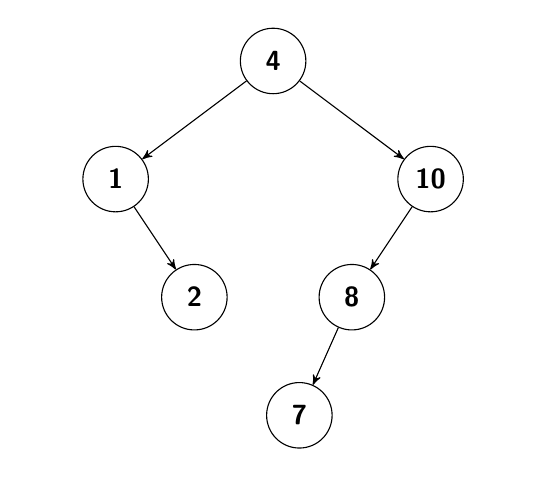
\begin{tikzpicture}[treenode/.style = {align=center, inner sep=1pt, text centered,
            font=\sffamily},
          bst/.style = {treenode, circle, black, font=\sffamily\bfseries, draw=black, text width=2em}, ->,>=stealth',level/.style={sibling distance = 4cm/#1,
          level distance = 1.5cm}]
        \node [bst] {4}
            child {node [bst] {1}
                child[edge from parent/.style={draw=none}] {node {}}
                child {node [bst](n6) {2}
                }
            }
            child {node (n10) [bst] {10}
               child {node [bst] {8}
                    child {node [bst] {7}}
                    child[edge from parent/.style={draw=none}] {node {}}
               }
               child[edge from parent/.style={draw=none}] {node {}}
            }
        ;
        \end{tikzpicture}
        \column{.59\textwidth}
       \faIcon{question-circle} Consider the following questions:
       
       \begin{itemize}
        \item Given a BST, what is time complexity of common operations (e.g., \texttt{search()}, \texttt{put()})?
        \item What is the height if inserting 1, 2, 4, 7, 8, and 10  sequentially?
       \end{itemize}
    \end{columns}

\end{frame}

\begin{frame}[fragile]

   \begin{columns}
    \column{.6\textwidth}
    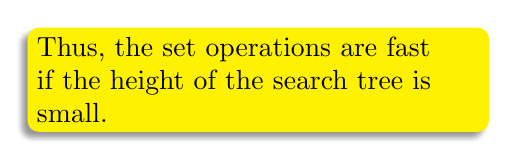
\begin{tikzpicture}
        \node[fill=yellow,blur shadow={shadow xshift=-0.5ex},
        text width=16em,anchor=south west,rounded corners]
        {Thus, the set operations
        are fast if the height of the search tree is small.};
    \end{tikzpicture}

    \begin{exampleblock}{Balanced Tree}
        A search tree is \alert{balanced} if it can guarantee that basic dynamic-set operations take $O(\lg{N})$ time in the worst case.
    \end{exampleblock} 
    \column{.39\textwidth}
    \begin{tikzpicture}[treenode/.style = {align=center, inner sep=.8pt, text centered,
        font=\sffamily},
      bst/.style = {treenode, circle, black, font=\sffamily\bfseries, draw=black, text width=1.8em}, ->,>=stealth',level/.style={sibling distance = 1.8cm,
      level distance = 1.2cm}]
    \node [bst] {1}
        child[edge from parent/.style={draw=none}] {node {}
        }
        child {node [bst] {2}
           child[edge from parent/.style={draw=none}] {node {}
           }
           child {node [bst] {4}
                child[edge from parent/.style={draw=none}] {node {}}
                child {node [bst] {7}
                   child[edge from parent/.style={draw=none}] {node {}}
                   child {node [bst] {8}
                     child[edge from parent/.style={draw=none}] {node {}
                       }
                     child {node [bst] {10}}
                   }
                }
           }
        }
    ;
    \end{tikzpicture}
\end{columns}

\end{frame}

\begin{frame}[fragile]
    \frametitle{1.2 Balanced Tree}
\begin{exampleblock}{Perfectly Height-balanced}
 A tree is \alert{perfectly} height-balanced if the left and right subtrees of any node are the same height.
\end{exampleblock}

\begin{columns}
    \column{.4\textwidth}<1->
    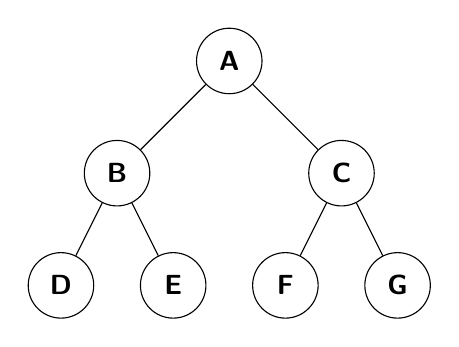
\begin{tikzpicture}[treenode/.style = {align=center, inner sep=1pt, text centered, font=\sffamily}, bst/.style = {treenode, circle, black, font=\sffamily\bfseries, draw=black, text width=2em},level/.style={sibling distance = 3cm/#1,
        level distance = 1.5cm}, scale=.95]
\node [bst] {A}
        child {node [bst] {B}
            child {node [bst] {D}}
            child {node [bst] {E}}
        }
        child {node [bst] {C}
            child {node [bst] {F}}
            child {node [bst] {G}}
        }
;
    \end{tikzpicture}     
    \column{.59\textwidth}<2->
    But \textbf{perfect height balance} is very rare: it is only possible if there are exactly $2^{H+1} - 1$ nodes.
\end{columns}

\end{frame}


\begin{frame}

    \section{\textcolor{darkmidnightblue}{2. AVL Tree}} 
    An AVL tree (named after inventors \textbf{A}delson-\textbf{V}elsky and \textbf{L}andis) is a self-balancing binary search tree (BST).
\end{frame}

\end{document}